\documentclass[11pt,a4paper]{article}

% --- Packages ---
\usepackage[utf8]{inputenc}
\usepackage[T1]{fontenc}
\usepackage{amsmath}
\usepackage{amssymb}
\usepackage{amsfonts}
\usepackage{geometry}
\usepackage{physics}
\usepackage{parskip}
\usepackage{cancel}
\usepackage[english]{babel}
\usepackage{tikz}
\usepackage{fancyhdr}
\usepackage{hyperref}
\usepackage{booktabs}
\usepackage{color}
\usetikzlibrary{patterns}
\usetikzlibrary{calc}

% --- Configuration de la page ---
\geometry{
    top=2.5cm,
    bottom=2.5cm,
    left=2.8cm,
    right=2.8cm,
    headheight=14pt
}

% --- En-têtes et pieds de page ---
\pagestyle{fancy}
\fancyhf{}
\lhead{\textit{Optical Refractive Index of Air Plasma}}
\rhead{\thepage}
\renewcommand{\headrulewidth}{0.5pt}
\renewcommand{\footrulewidth}{0pt}

% --- Commandes pour les vecteurs en colonne ---
\newcommand{\vectII}[2]{%
    \begin{pmatrix}
    #1 \\
    #2
    \end{pmatrix}%
}

\newcommand{\vectIII}[3]{%
    \begin{pmatrix}
    #1 \\
    #2 \\
    #3
    \end{pmatrix}%
}

% --- Titre du document ---
\title{\textbf{Optical Refractive Index of Air Plasma}}
\author{Anatole Cremel--Schlemer}
\date{April 14, 2026}

\begin{document}

\maketitle
\thispagestyle{fancy}


\tableofcontents
\newpage

%============================================================================
\section{Two-Plane-Wave Interferometry}
%============================================================================

The Nomarski interferometer can be understood as a configuration that allows retrieval of phase information about a medium under investigation. We derive the fundamental equations governing the interference pattern produced by two plane waves with different propagation directions.

\subsection{Field Configuration and Wave Vectors}

Consider two plane waves propagating in the same medium with refractive index $\eta_i$:
\begin{equation}
E_1 = \underline{E_0} \, e^{i(\vec{k}_1 \cdot \vec{r} - \omega t)}
\end{equation}
\begin{equation}
E_2 = \underline{E_0} \, e^{i(\vec{k}_2 \cdot \vec{r} - \omega t)}
\end{equation}

where the wave vectors are defined as:
\begin{equation}
\vec{k}_1 = \frac{2\pi}{\lambda}\eta_i \vectIII{\sin{\theta}}{0}{\cos{\theta}} = k \vectIII{\sin{\theta}}{0}{\cos{\theta}}
\end{equation}
\begin{equation}
\vec{k}_2 = \frac{2\pi}{\lambda}\eta_i \vectIII{-\sin{\theta}}{0}{\cos{\theta}} = k \vectIII{-\sin{\theta}}{0}{\cos{\theta}}
\end{equation}

These two plane waves propagate symmetrically with respect to the normal axis, making an angle $2\theta$ with each other. In order to take into account the symmetry by rotation around the $z$-axis, we introduce an arbitrary angle $\phi$ through the rotation operator:
$$\mathcal{R}_z(\phi) = \begin{pmatrix}
\cos\phi & -\sin\phi & 0 \\
\sin\phi & \cos\phi & 0 \\
0 & 0 & 1
\end{pmatrix}$$

Applying it to $\vec{k}_1$ and $\vec{k}_2$:
$$
\vec{k}_1 \xrightarrow{\mathcal{R}_z(\phi)} k \vectIII{\cos{\phi}\sin{\theta}}{\sin{\phi}\sin{\theta}}{\cos{\theta}}
$$

$$
\vec{k}_2 \xrightarrow{\mathcal{R}_z(\phi)} k \vectIII{-\cos{\phi}\sin{\theta}}{-\sin{\phi}\sin{\theta}}{\cos{\theta}}
$$

\subsection{Intensity Distribution}
Setting the observation screen such that it is located at $z = 0$.
The intensity observed at a point on the screen is then given by:
\begin{align}
I(x,y) = \big\langle|\vec{\underline{E}}|^2\big\rangle = \big\langle|\vec{\underline{E_1}}|^2\big\rangle + \big\langle|\vec{\underline{E_2}}|^2\big\rangle + \big\langle \vec{\underline{E_1}}\vec{\underline{E_2}}^* +\vec{\underline{E_1}}^*\vec{\underline{E_2}} \big\rangle\\
I(x,y) = I_1 + I_2 + \sqrt{I_1I_2} \cos\big((\vec{k}_1 - \vec{k}_2) \cdot \vec{r}\big)
\end{align}

For equal amplitudes, this simplifies to:
\begin{equation}
I(x,y) = 2I_0(x,y)\left[1 + \cos\big((\vec{k}_1 - \vec{k}_2) \cdot \vec{r}\big)\right]
\end{equation}

\subsection{Fringe Spacing and Spatial Frequency}

Computing the phase difference:
\begin{equation}
(\vec{k}_1 - \vec{k}_2) \cdot \vec{r} = k \left[ \vectIII{\cos{\phi}\sin{\theta}}{\sin{\phi}\sin{\theta}}{\cos{\theta}}-\vectIII{-\cos{\phi}\sin{\theta}}{-\sin{\phi}\sin{\theta}}{\cos{\theta}}\right] \cdot \vectIII{x}{y}{0} = 2k\sin{\theta}\bigg[x\cos{\phi}+y\sin{\phi}\bigg]
\end{equation}
The intensity equation reads: 
\begin{equation}
I(x,y) = 2I_0\left[1 + \cos\!\big(2k\sin{\theta}(x\cos\phi + y\sin\phi)\big)\right]
\end{equation}
The fringes reach maximum intensity when the phase of the cosine is a multiple of $2\pi$.
The interference pattern is composed of fringes rotated of an angle $\phi$ around the $z$-axis. Setting the right coordinates, it is possible to calculate the distance between two successive fringes. Plugging $ x=R\cos{\phi}$ and $y=\sin{\phi}$ : 
\begin{equation}
R = \frac{\lambda}{2\sin\theta} = \frac{1}{\nu_0}.
\end{equation}
Where $\nu_0$ is the spatial-carrier frequency of the fringes along the tilted axis.

\begin{equation}
\boxed{I(x,y) = 2I_0(x,y)\left[1 + \cos\big(2\pi \nu_0(x\cos{\phi}+y\sin{\phi}\big)\right]}
\end{equation}

\begin{figure}[h!]
    \centering
    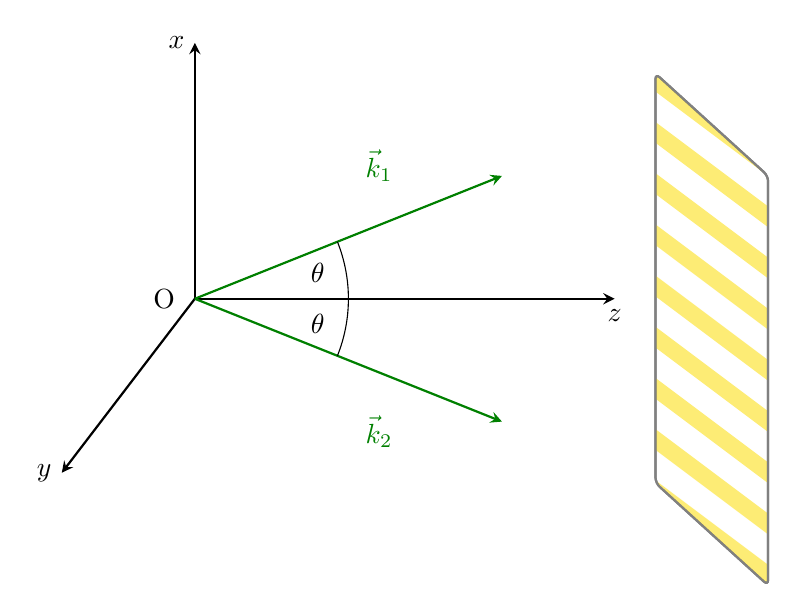
\begin{tikzpicture}[scale=1.3]
        % Axes 3D (Perspective isométrique simulée)
        \draw[-stealth, thick] (0,0) -- (0,2.5) node[left] {$x$};
        \draw[-stealth, thick] (0,0) -- (-1.3,-1.7) node[left] {$y$};
        \draw[-stealth, thick] (0,0) -- (4.1,0) node[below] {$z$};

        % Label de l'origine
        \node[left] at (-0.1, 0) {O};

        % ---------------------------------------------------
        % ÉCRAN ET FRANGES D'INTERFÉRENCE
        % ---------------------------------------------------
        \def\screen{
            (4.5, 2.2) -- (5.6, 1.2) -- (5.6, -2.8) -- (4.5, -1.8) -- cycle
        }
        
        \draw[gray, thick, fill=white, rounded corners=2pt] \screen;

        \begin{scope}
            \clip[rounded corners=2pt] \screen;
            \foreach \i in {-4,-3.5,...,4} {
                \draw[yellow!80!orange, line width=6pt, opacity=0.55] (4, \i) -- (6, \i-1.5);
            }
        \end{scope}

        \draw[gray, thick, rounded corners=2pt] \screen;

        % ---------------------------------------------------
        % VECTEURS D'ONDE ET ANGLES
        % ---------------------------------------------------
        \draw[-stealth, thick, green!50!black] (0,0) -- (3, 1.2);
        \node[green!50!black] at (1.8, 1.3) {$\vec{k}_1$};

        \draw[-stealth, thick, green!50!black] (0,0) -- (3, -1.2);
        \node[green!50!black] at (1.8, -1.3) {$\vec{k}_2$};

        % Arcs et angles
        \draw (1.5,0) arc (0:21.8:1.5);
        \node at (1.2, 0.25) {$\theta$};

        \draw (1.5,0) arc (0:-21.8:1.5);
        \node at (1.2, -0.25) {$\theta$};

    \end{tikzpicture}
    \caption{Interference of two plane waves propagating symmetrically with an angle $2\theta$, creating an interference pattern on the screen (shown for $\phi = 0$).}
    \label{fig:interference}
\end{figure}

%============================================================================
\section{Phase and Amplitude Extraction via Fourier Analysis}
%============================================================================

\subsection{Principles \& Comparative Advantages}

Nomarski interferograms read:
\begin{equation}
    I(x,y) = a(x,y) + b(x,y)\cos\!\big[2\pi\nu_0 x + \varphi(x,y)\big]
\end{equation}
$a(x,y)$ is the background term, $b(x,y)$ the amplitude modulation term, and $\varphi(x,y)$ the phase of interest. Using Euler's formula, this can be rewritten as:
\begin{equation}
I(x,y) = a(x,y) + c(x,y)e^{i2\pi\nu_0 x} + c^*(x,y)e^{-i2\pi\nu_0 x}
\end{equation}
with the complex modulation function
\begin{equation}
    c(x, y) = \tfrac{1}{2}b(x, y)e^{i\varphi(x, y)}
\end{equation}

Whereas, in conventional contour-fringe interferometry interferograms ($\nu_0 = 0$) the intensity reads : $$I(x,y) = a(x,y) + b(x,y)\cos\varphi(x,y)$$
$a$, $b$ and $\varphi$ are mixed which limits accuracy. Moreover, the parity of the cosine prevents determining the sign of $\varphi$. This is a major drawback in plasma diagnostics, where $\varphi(x,y)$ is proportional to the line-integrated electron density allowing to distinguishes compressed from rarefied regions of the plasma.
\begin{equation}
\varphi(x,y) \propto \int n_e(x,y,z)\,\mathrm{d}z,
\end{equation}

The Takeda method~\cite{takeda1982fourier} overcomes both limitations through a spatial homodyne demodulation. As in classical heterodyne detection, the signal of interest is carried by an oscillating reference, here the spatial carrier $\nu_0$, generated by the tilted $2\theta$ incidence angle of the interferometer arms. Multiplying by this reference (equivalently, bandpass filtering around $+\nu_0$ in the Fourier plane) shifts the sideband down to baseband and yields the complex modulation $c(x,y) = \tfrac{1}{2}b(x,y)e^{i\varphi(x,y)}$. The background $a(x,y)$ is filtered out with the DC lobe (background), while $b(x,y)$ and $\varphi(x,y)$ end up respectively in the modulus and argument of $c(x,y)$, and are therefore fully separated.

This configuration improves the sensitivity to weak phase variations. In contour interferometry, small variation around the reference weakly affect the intensity since the variations lie around the extremum of a cosine function. Thus, a small phase $\varphi \ll 1$ modifies the intensity quadratically limiting the identification of small index change.
$$
\Delta I_{contour}(x,y) \approx  \frac{b(x,y)}{2}\varphi^2(x,y)
$$
In the Takeda method, expanding the cosine around the carrier gives
$$
\Delta I_{Takeda}(x,y)  \approx -b(x,y)\sin{(2\pi\nu_0 x)}\,\,\varphi(x,y)
$$ 
$\varphi(x,y)$ modulates the fringe pattern linearly. This linear response to small phases is what allows sub-wavelength sensitivity, as reported in~\cite{takeda1982fourier}.

These properties make the method particularly adapted to laser-produced plasmas. Takeda operates on a single interferogram. Furthermore, the probe beam is strongly affected by refraction, absorption and self-emission, all of which corrupt $a(x,y)$ and $b(x,y)$, variations that the method naturally rejects.

\subsection{Application to Reference and Measurement Interferograms}

We consider two interferograms: a background reference acquired without plasma, and a measurement with plasma. To account for the arbitrary orientation of the carrier fringes, we introduce $\alpha = \cos\phi$, $\beta = \sin\phi$. The two interferograms read:
\begin{align}
I_{\text{ref}}(x,y)  &= a_1(x,y) + b_1(x,y)\cos\!\big(2\pi\nu_0 (\alpha x + \beta y)\big) \\
I_{\text{meas}}(x,y) &= a_2(x,y) + b_2(x,y)\cos\!\big(2\pi\nu_0 (\alpha x + \beta y) + \varphi(x,y)\big)
\end{align}

Introducing the complex modulation functions
\begin{equation}
c_1(x,y) = \tfrac{1}{2}b_1(x,y), \qquad c_2(x,y) = \tfrac{1}{2}b_2(x,y)\,e^{i\varphi(x,y)},
\end{equation}
they can be written compactly as:
\begin{align}
I_{\text{ref}}(x,y)  &= a_1(x,y) + c_1(x,y)\,e^{i2\pi\nu_0(\alpha x+\beta y)} + c_1^*(x,y)\,e^{-i2\pi\nu_0(\alpha x+\beta y)} \\
I_{\text{meas}}(x,y) &= a_2(x,y) + c_2(x,y)\,e^{i2\pi\nu_0(\alpha x+\beta y)} + c_2^*(x,y)\,e^{-i2\pi\nu_0(\alpha x+\beta y)}
\end{align}

\subsection{Fourier Transform and Phase Extraction}

Applying the 2D Fourier transform,
$$
\hat{f}(\nu_x,\nu_y) = \iint f(x,y)\,e^{-i2\pi(\nu_x x + \nu_y y)}\,\mathrm{d}x\,\mathrm{d}y,
$$
together with the frequency-shift theorem
$$
\mathcal{F}\!\left[f(x,y)\,e^{i2\pi\nu_0(\alpha x+\beta y)}\right](\nu_x,\nu_y) = \hat{F}(\nu_x - \alpha\nu_0,\ \nu_y - \beta\nu_0),
$$
we obtain:
\begin{align}
\hat{I}_{\text{ref}}(\nu_x,\nu_y)  &= \hat{A}_1(\nu_x,\nu_y) + \hat{C}_1(\nu_x - \alpha\nu_0,\ \nu_y - \beta\nu_0) + \hat{C}_1^*(\nu_x + \alpha\nu_0,\ \nu_y + \beta\nu_0) \\
\hat{I}_{\text{meas}}(\nu_x,\nu_y) &= \hat{A}_2(\nu_x,\nu_y) + \hat{C}_2(\nu_x - \alpha\nu_0,\ \nu_y - \beta\nu_0) + \hat{C}_2^*(\nu_x + \alpha\nu_0,\ \nu_y + \beta\nu_0)
\end{align}

Note that although the phase $\varphi(x,y)$ appears inside the cosine argument alongside the carrier term, it does not produce a frequency shift in the Fourier plane: being a spatial function rather than a constant frequency, it is embedded in the structure of $\hat{C}_2$, not in its position. Provided that $a_{1,2}$, $b_{1,2}$ and $\varphi$ vary slowly compared to $\nu_0$, the three lobes of each spectrum are well separated and can be isolated individually.

A bandpass filter centred on the positive sideband at $(\alpha\nu_0,\ \beta\nu_0)$ yields:
\begin{align}
\hat{I}_{\text{ref,filt}}(\nu_x,\nu_y)  &= \hat{C}_1(\nu_x - \alpha\nu_0,\ \nu_y - \beta\nu_0) \\
\hat{I}_{\text{meas,filt}}(\nu_x,\nu_y) &= \hat{C}_2(\nu_x - \alpha\nu_0,\ \nu_y - \beta\nu_0)
\end{align}

An inverse Fourier transform then gives:
\begin{align}
I_{\text{ref,filt}}(x,y)  &= \tfrac{1}{2}b_1(x,y)\,e^{i2\pi\nu_0(\alpha x+\beta y)} \\
I_{\text{meas,filt}}(x,y) &= \tfrac{1}{2}b_2(x,y)\,e^{i\big(2\pi\nu_0(\alpha x+\beta y) + \varphi(x,y)\big)}
\end{align}

\subsection{Phase and Transmittance Retrieval}

The complex ratio of the two filtered signals cancels the carrier:
\begin{equation}
z(x,y) \equiv \frac{I_{\text{meas,filt}}(x,y)}{I_{\text{ref,filt}}(x,y)} = \frac{b_2(x,y)}{b_1(x,y)}\,e^{i\varphi(x,y)}
\end{equation}

Writing $z = a + ib$ with $a, b \in \mathbb{R}$, the \emph{transmittance} of the plasma is recovered from the modulus squared,
\begin{equation}
T(x,y) = |z(x,y)|^2 = \frac{b_2^2(x,y)}{b_1^2(x,y)},
\end{equation}
and the phase from the two-argument arctangent:
\begin{equation}
\boxed{\ \varphi(x,y) = \operatorname{atan2}(\Im{(z(x,y))},\Re{(z(x,y)})\ }
\end{equation}

Using a reference interferogram, rather than extracting $\arg(I_{\text{meas,filt}})$ directly, has the advantage of removing any residual phase tilt or distortion arising from optical misalignments of the carrier, yielding the plasma-induced phase $\varphi(x,y)$ alone.
%============================================================================
\section{Digital Recording and Phase Shift Correction}
%============================================================================
\usetikzlibrary{decorations.pathmorphing, arrows.meta, angles, quotes}

\subsection{Spatial and Frequential Resolutions}
\subsubsection{Nyquist Frequency Limit}
We've seen the principles of the Takeda method to recover fine phase information by modulating spatial frequency via a Wollaston cube. However to be able to observe very fine detuning we need to use digital analysis and therefore use a camera sensor to capture the holographic interference pattern. 
This conversion from continuous to discrete signals (analogue to digital) comes with some limitations we will try to explain in this section.

The first limitation comes from the Nyquist frequency limit. On a discret sample, the shortest oscillation that can be observed without aliasing effect, has to spread on two pixels, an alternance of high and low value of the light intensity. The shortest period observed is then limited by the size of these two successive pixels. Thus the Nyquist frequency limit is defined as $$\nu_N= \frac{1\,\text{period} }{2 \, \text{pixels}}= \frac{1}{2\Delta x}\, \, \, \,  \text{with} \, \Delta x = \text{pixel size}$$
However with a 45° orientation of successive fringes, the value of successive pixels can be calculated from a continuous intensity function $\cos^2(2\pi f_x x +2\pi f_y y +\phi) $ as : 
$$I(n_x,n_y) = \int^{n_x+\frac{1}{2}}_{n_x-\frac{1}{2}}\int^{n_y+\frac{1}{2}}_{n_y-\frac{1}{2}}\cos^2(2\pi f_x x +2\pi f_y y +\phi)\, dx \,dy $$
$$ I(n_x, n_y) = \frac{1}{2} + \frac{1}{2} \cos(2\pi f_x n_x + 2\pi f_y n_y +\phi) \left[ \frac{\sin(\pi f_x)}{\pi f_x} \right] \left[ \frac{\sin(\pi f_y)}{\pi f_y} \right] $$
With $f_x = f_y = \frac{1}{2}$:
$$ I(n_x, n_y) = \frac{1}{2} + \frac{1}{2} \cos(\pi (n_x + n_y)+\phi) \left[ \frac{\sin(\pi/2)}{\pi/2} \right] \left[ \frac{\sin(\pi/2)}{\pi/2} \right] = \frac{1}{2} +\frac{2}{\pi^2}\cos{(\pi(n_x+n_y)+\phi)} $$
This function is maximum for $\phi = 0$ and pixel value alternates between two value  $$\frac{1}{2} \pm \frac{2}{\pi^2}$$
\begin{figure}[h]
    \centering
    
\includegraphics[width=0.41\linewidth]{pixel value.png}
    \caption{Exact Spatial Integration over Square Pixels at Nyquist Limit (45°)}
    \label{fig:pixel}
\end{figure}

\subsubsection{Sample Diffraction and Smallest Resolved Feature}
On the other hand, the highest spatial frequency transmitted by the optical system is limited by the size of the smallest feature of the sample we try to capture. 
The plasma acts as a diffracting object for incident light beams. The first order deflection angle is given by the path difference $\Delta l = d\sin{\theta}$, where $d$ is the caracteristic size of the diffracted object.
The corresponding detuning term reads : $$k\Delta l = \frac{2\pi}{\lambda}d\sin{\theta}$$
Constructive interference between contributions of successive periods of the diffracting object occurs when $k\Delta l = m2\pi$, defining the diffraction orders.
In the case of a first order diffraction $m = \pm 1$: Thus the first order diffracted beam originating from a $d$ sized feature are coming with an angle $\theta$ onto the microscop lense such that $\sin{\theta} = \frac{\lambda}{d}$.

\begin{tikzpicture}

% --- ONDES INCIDENTES ---
\foreach \x in {-4, -3.2, -2.4, -1.6, -0.8} {
    \draw[decorate, decoration={snake, amplitude=0.35mm, segment length=2.5mm}, thin] (\x, 2.5) -- (\x, -2.5);
}

% Flèche de direction
\draw[thick, fill=white, line join=round] (-3.6, -0.5) -- (-2.0, -0.5) -- (-2.0, -0.9) -- (-1.0, 0) -- (-2.0, 0.9) -- (-2.0, 0.5) -- (-3.6, 0.5) -- cycle;

% --- OBSTACLE ET FENTE ---
\fill[black!90] (0, 1.2) rectangle (0.35, 4);
\fill[black!90] (0, -1.2) rectangle (0.35, -4);

% Indication de la largeur d
\draw[<->, >=stealth, thick] (-0.3, 0.2) -- (-0.3, -0.2) node[midway, left] {$d$};
\draw[thin, gray] (-0.6, 1.2) -- (0, 1.2);
\draw[thin, gray] (-0.6, -1.2) -- (0, -1.2);

% Ligne pointillée (ouverture)
\draw[densely dashed, thick] (0, 1.2) -- (0, -1.2);

% --- RAYONS DIFFRACTÉS ---
% Définition de l'angle de déviation
\def\angleDev{26} 

\foreach \y in {1.0, 0.75, 0.5, 0.25, 0, -0.25, -0.5, -0.75, -1.0} {
    % Ordre +1
    \draw[-{Stealth[length=2.5mm, width=1.5mm]}, blue!70!black, thin] (0, \y) -- ++(\angleDev:7.5);
    
    % Ordre 0 (Central)
    \draw[-{Stealth[length=2.5mm, width=1.5mm]}, black, thin] (0, \y) -- ++(0:7.5);
    
    % Ordre -1
    \draw[-{Stealth[length=2.5mm, width=1.5mm]}, blue!70!black, thin] (0, \y) -- ++(-\angleDev:7.5);
}

% --- INDICATION DE L'ANGLE THETA ---
% On définit des points pour tracer l'angle
\coordinate (A) at (0,0);
\coordinate (B) at (5,0);
\coordinate (C) at (5, {5*tan(\angleDev)});

\draw[thick, red!80!black] (4,0) arc (0:\angleDev:4) node[midway, right, xshift=2pt] {$\theta$};

% Labels des ordres
\node[right] at (7.5, {7.5*tan(\angleDev)}) {\small 1rst Order};
\node[right] at (7.5, 0) {\small 0th Order};
\node[right] at (7.5, {-7.5*tan(\angleDev)}) {\small -1rst Order};

\end{tikzpicture}


We can then invert the problem: what is the size of the smallest feature a microscope lens can resolve, knowing that the maximum acceptance angle is given by the numerical aperture? $$NA = n \sin{\alpha}\xrightarrow{n_{air}=1}\sin{\alpha}$$
For the first order diffracted beam to be collected by the lens, one must have $\sin{\theta}\leq\sin{\alpha}$, which gives the shortest resolved feature in our coherent on-axis configuration : $$R_0= \frac{\lambda}{\sin{\alpha}} = \frac{\lambda}{NA}$$
\begin{tikzpicture}

% --- ONDES INCIDENTES ---
% Décalées plus à gauche pour libérer de l'espace
\foreach \x in {-5.2, -4.4, -3.6, -2.8, -2.0} {
    \draw[decorate, decoration={snake, amplitude=0.35mm, segment length=2.5mm}, thin] (\x, 2.5) -- (\x, -2.5);
}

% Indication de la longueur d'onde \lambda
\draw[<->, >=stealth, thick] (-3.6, 2.2) -- (-2.8, 2.2) node[midway, above] {$\lambda$};

% Flèche de direction (reculée vers la gauche)
\draw[thick, fill=white, line join=round] (-4.0, -0.5) -- (-2.2, -0.5) -- (-2.2, -0.9) -- (-1.2, 0) -- (-2.2, 0.9) -- (-2.2, 0.5) -- (-4.0, 0.5) -- cycle;

% --- OBSTACLE ET FENTE ---
\fill[black!90] (0, 1.2) rectangle (0.35, 4);
\fill[black!90] (0, -1.2) rectangle (0.35, -4);

% Lignes de rappel grises (allongées pour s'adapter au texte)
\draw[thin, gray] (-1.0, 1.2) -- (0, 1.2);
\draw[thin, gray] (-1.0, -1.2) -- (0, -1.2);

% Ligne pointillée (ouverture)
\draw[densely dashed, thick] (0, 1.2) -- (0, -1.2);

% --- COTES d ET R0 ---
% Indication de la largeur d
\draw[<->, >=stealth, thick, orange] (-0.3, 0.2) -- (-0.3, -0.2) node[midway, left=4pt] {$R_0$};

% Indication de R_0 et sa formule en orange
% J'ai allongé un peu la flèche et décalé le texte (left=4pt) pour qu'il soit bien lisible
\draw[<->, >=stealth, thick] (-0.3, 1.1) -- (-0.3, 0.3) node[midway, left=4pt] {$d$};


% --- RAYONS DIFFRACTÉS ---
% Définition de l'angle de déviation
\def\angleDev{26} 

\foreach \y in {0} {
    % Ordre +1
    \draw[-{Stealth[length=2.5mm, width=1.5mm]}, blue!70!black, thick] (0, \y) -- ++(\angleDev:8.5);
    
    % Ordre 0 (Central)
    \draw[-{Stealth[length=2.5mm, width=1.5mm]}, black, thick] (0, \y) -- ++(0:8.5);
    
    % Ordre -1
    \draw[-{Stealth[length=2.5mm, width=1.5mm]}, blue!70!black, thick] (0, \y) -- ++(-\angleDev:8.5);
}

% --- LENTILLE ---
\def\lensX{6.5}
\def\lensY{4.0}
% Dessin de la lentille biconvexe
\draw[thick, fill=cyan!10, opacity=0.8] (\lensX, \lensY) to[bend left=15] (\lensX, -\lensY) to[bend left=15] cycle;
% Axe principal de la lentille
\draw[dash dot, thin, gray] (\lensX, \lensY+0.5) -- (\lensX, -\lensY-0.5);

% --- OUVERTURE NUMÉRIQUE (NA) ---
% Rayons marginaux définissant l'ouverture de la lentille
\draw[densely dashed, thick, orange!90!black] (0,0) -- (\lensX, \lensY);
\draw[densely dashed, thick, orange!90!black] (0,0) -- (\lensX, -\lensY);

% Calcul et tracé de l'angle Alpha
\pgfmathsetmacro{\angleAlpha}{atan(\lensY/\lensX)}
\draw[thick, orange!90!black] (4.5,0) arc (0:\angleAlpha:4.5) node[midway, right, xshift=2pt, yshift=4pt] {$\alpha$};

% Label NA 
\node[orange!90!black, right] at (\lensX-4.5, \lensY-0.5) {$\mathrm{NA} = \sin \alpha = \frac{\lambda}{R_0}$};

% --- INDICATION DE L'ANGLE THETA ET DE LA FORMULE ---
\draw[thick, red!80!black] (2,0) arc (0:\angleDev:2) node[midway, right, xshift=2pt] {$\theta \left( \sin\theta = \frac{\lambda}{d} \right)$};

% --- LABELS DES ORDRES ---
\node[right] at (8, {7.8*tan(\angleDev)}) {\small 1rst Order};
\node[right] at (8.5, 0) {\small 0th Order};
\node[right] at (8, {-7.8*tan(\angleDev)}) {\small -1rst Order};

\end{tikzpicture}


The more familiar Abbe formula $\tfrac{\lambda}{2NA}$ comes from tilting the illumination instead of using an axial beam. If the sample is illuminated under an angle $\alpha$, the 0th order is rejected at $-\alpha$ and a first order can still enter the lens up to $\sin\theta = 2\sin\alpha$, doubling the bandwidth. Standard microscopes reach this limit naturally with a Köhler condenser that fills the whole cone $[-\alpha,+\alpha]$. Our setup uses a coherent on-axis beam, so the resolution stays at $\tfrac{\lambda}{NA}$.

\textbf{TO be edited}

The image is then magnified via a $4f$ optical system, and thus the final smallest resolved feature visible on the sensor has a width of $R_s=M_{tot}R_0$.

In the frequency domain, the optical system acts as a low-pass filter whose cutoff is the highest spatial frequency transmitted to the sensor : $$\nu_{max} = \frac{1}{R_s}= \frac{1}{M_{tot}R_0}= \frac{NA}{M_{tot}\lambda}$$
For the digital recording not to lose any of this optical bandwidth, the Nyquist frequency of the sensor must satisfy $\nu_N\geq\nu_{max}$.

\subsection{Off-axis Digital Holography}
Off-axis holography was proposed by Leith and Upatnieks ~\cite{Leith}. Recalling formula (6): 
$$I(x,y) = |\underline{E_1}|^2 + |\underline{E_2}|^2  + 2|\underline{E_1E_2}| \cos\big(2\pi\nu_0(\alpha x + \beta y)\big)$$
We develop the cosine using Euler's identity :
$$I(x,y) = |\underline{E_1}|^2 + |\underline{E_2}|^2  + |\underline{E_1E_2}| e^{i2\pi\nu_0(\alpha x + \beta y)} +|\underline{E_1E_2}|e^{-i2\pi\nu_0(\alpha x + \beta y)}$$
Such a calculation exhibits translation operators along x and y direction within the expression of the holographic pattern : $ \mathcal{T}_{\alpha\nu_0} = e^{-i2\pi(\alpha\nu_0) x}$.
These operators act as translation operators in the Fourier domain : $\mathcal{F}[\mathcal{T}_A f(x)](\nu) =F(\nu-A)$
Applying the Fourier transform to $ I(x,y)$ :
\begin{align}
\begin{split}
\mathcal{I}(\nu_x,\nu_y) = \mathcal{F}[|\underline{E_1}|^2] + \mathcal{F}[|\underline{E_2}|^2] + \mathcal{F}[|\underline{E_1E_2}|](\nu_x-\alpha\nu_0,\, \nu_y -\beta\nu_0) \\+ \mathcal{F}[|\underline{E_1E_2}|](\nu_x+\alpha\nu_0,\, \nu_y +\beta\nu_0) 
\end{split}
\end{align}
The two first terms are called the DC components and encode the low frequency of the signal. The Two last terms are called the carrier components, they carry precious informations about the high frequencies, that are relevant in our case because the variation of the refractive index are very local to the impact spot.
Thus in the case of same intensity beam, 
$$\mathcal{I}(\nu_x,\nu_y) = 2 \mathcal{F}[|E|^2] + \mathcal{F}[|E|^2](\nu_x-\alpha\nu_0,\nu_y-\beta\nu_0)+ \mathcal{F}[|E|^2](\nu_x+\alpha\nu_0,\nu_y+\beta\nu_0)$$
Since the highest spatial frequency transmitted by the optics is $\nu_{max}=\frac{NA}{M_{tot}\lambda}$, the support of $\mathcal{F}[E]$ is a disk of radius $\nu_{max}$. The DC term is an autocorrelation $\mathcal{F}[|E|^2] = \mathcal{F}[E] \circledast \mathcal{F}[E^*]$, whose support has radius $2\nu_{max}$

\textbf{Problem the carrier has same bandwidth....}

\textbf{INSERT DFT Method explainations}


%============================================================================
\section{Abel Transform and Refractive Index Reconstruction}
%============================================================================

\subsection{Physical Setup and Phase Accumulation}

The Abel transform is the key mathematical tool for reconstructing the refractive index from the measured phase distribution. Consider the physical setup: two plane waves ($E_{\text{ref}}$ and $E_{\text{probe}}$) interfere in a Nomarski interferometer. The probe beam propagates through an air plasma, acquiring a phase shift $\Delta\phi(x,z)$ relative to the reference beam.

These plane waves propagate in opposite directions along the $y$-axis. We write:
\begin{align}
E_{\text{ref}} &= \underline{E_0} \, e^{-ik\int \eta_{\text{air}} \, dy} = \underline{E_0} \, e^{-iky} \\
E_{\text{probe}} &= \underline{E_0} \, e^{-ik \int \eta(x,y,z) \, dy}
\end{align}

where $\eta(x,y,z)$ is the complex refractive index of the air plasma.

\subsection{Cylindrical Symmetry}

Since the air plasma exhibits approximate cylindrical symmetry along the $z$-axis, the refractive index can be expressed using cylindrical coordinates with $r = \sqrt{x^2 + y^2}$:
\begin{equation}
E_{\text{probe}} = \underline{E_0} \, e^{-i2k\int_0^{\infty} \eta(r,z) \, dy}
\end{equation}

The phase difference between the reference and probe beams is:
\begin{equation}
\phi(x,z) = \frac{2\pi}{\lambda_L}\left[2\int_0^{\infty}\eta(r,z) \, dy - 2\int_0^{\infty}1 \, dy\right]
\end{equation}

\subsection{Derivation of the Abel Transform}

Simplifying and expressing in terms of the refractive index deviation:
\begin{equation}
\phi(x,z) = 2\left(\frac{2\pi}{\lambda_L}\right)\int_0^{\infty}[\eta(r,z) - 1] \, dy
\end{equation}

Using the substitution $y = \sqrt{r^2 - x^2}$ and $dy = \frac{r \, dr}{\sqrt{r^2 - x^2}}$:
\begin{equation}
\phi(x,z) = 2\left(\frac{2\pi}{\lambda_L}\right)\int_x^{\infty} \frac{[\eta(r,z) - 1] \, r}{\sqrt{r^2 - x^2}} \, dr
\end{equation}

This is consistent with equation (4) of reference~\cite{gonzalez2012plasma}.

\subsection{Inverse Abel Transform}

To retrieve the refractive index, we invert this relation using the inverse Abel transform. Let:
\begin{align}
f(r) &= \eta(r,z) - 1 \\
F(x) &= \frac{\lambda_L}{4\pi}\phi(x,z)
\end{align}

The forward Abel transform is:
\begin{equation}
F(x) = 2\int_x^{\infty} \frac{f(r) \, r}{\sqrt{r^2 - x^2}} \, dr
\end{equation}

The inverse transform is obtained by applying the integral operator $\int_{\rho}^{\infty} \frac{x \, dx}{\sqrt{x^2 - \rho^2}}$ to both sides and using the identity $\int_{\rho}^{r} \frac{x \, dx}{\sqrt{(r^2-x^2)(x^2-\rho^2)}} = \frac{\pi}{2}$.

After differentiation with respect to the parameter $\rho$, the inverse Abel transform becomes:
\begin{equation}
f(\rho) = -\frac{1}{\pi} \int_{\rho}^{\infty} \frac{dF(x)/dx}{\sqrt{x^2 - \rho^2}} \, dx
\end{equation}

Substituting back the definitions of $f$ and $F$:
\begin{equation}
\boxed{\eta(r,z) = 1 - \frac{1}{\pi}\left(\frac{\lambda_L}{2\pi}\right)\int_r^{\infty} \frac{d\phi(x,z)/dx}{\sqrt{x^2 - r^2}} \, dx}
\end{equation}

\subsection{Key Abel Transform Relations}

For reference, the fundamental forward and inverse relations are:
\begin{equation}
\boxed{F(x) = 2\int_x^{\infty} \frac{f(r) \, r}{\sqrt{r^2 - x^2}} \, dr}
\end{equation}

\begin{equation}
\boxed{f(\rho) = -\frac{1}{\pi} \int_{\rho}^{\infty} \frac{dF(x)/dx}{\sqrt{x^2 - \rho^2}} \, dx}
\end{equation}

%============================================================================
\section{Numerical Implementation}
%============================================================================

\subsection{Trapezoidal Rule for Numerical Integration}

To compute the inverse Abel transform numerically, we employ the trapezoidal rule for evaluating the integral. The method consists of approximating the integral as a sum of trapezoidal areas. For the interval $[x_k, x_{k+1}]$:

\begin{equation}
A_k \equiv \int_{x_k}^{x_{k+1}} g(x) \, dx \approx \frac{1}{2}(x_{k+1} - x_k)[g(x_{k+1}) + g(x_k)]
\end{equation}

\subsection{Discrete Formulation}

In our case, the integrand is:
\begin{equation}
g(x_k, r_i) = \frac{d F(x)/dx\big|_{x=x_k}}{\sqrt{x_k^2 - r_i^2}}
\end{equation}

Assuming a constant integration step $\Delta x = x_{k+1} - x_k$. To avoid the mathematical singularity at $x = r_i$, the numerical integration begins at the next pixel (index $k = i+1$). The discrete integral becomes:

\begin{equation}
f(r_i) = -\frac{1}{\pi}\sum_{k=i+1}^{N-2} A_k = -\frac{\Delta x}{2\pi}\sum_{k=i+1}^{N-2} \left[ g(x_{k+1}, r_i) + g(x_k, r_i) \right]
\end{equation}

\subsection{Spatial Derivative Approximation}

Substituting the full expression for $g(x_k, r_i)$:
\begin{equation}
f(r_i) = -\frac{\Delta x}{2\pi}\sum_{k=i+1}^{N-2} \left[ \frac{dF(x)/dx\big|_{x=x_{k+1}}}{\sqrt{x_{k+1}^2 - r_i^2}} + \frac{dF(x)/dx\big|_{x=x_k}}{\sqrt{x_k^2 - r_i^2}} \right]
\end{equation}

To approximate the spatial derivative, we use the Euler forward-difference formula:
\begin{equation}
\frac{dF(x)}{dx}\bigg|_{x=x_k} \approx \frac{F(x_{k+1}) - F(x_k)}{\Delta x}
\end{equation}

\subsection{Simplified Numerical Formula}

Substituting this approximation, the constant spatial step $\Delta x$ cancels perfectly:

\begin{equation}
\boxed{f(r_i) = -\frac{1}{2\pi}\sum_{k=i+1}^{N-2} \left[ \frac{F(x_{k+2}) - F(x_{k+1})}{\sqrt{x_{k+1}^2 - r_i^2}} + \frac{F(x_{k+1}) - F(x_k)}{\sqrt{x_k^2 - r_i^2}} \right]}
\end{equation}

This formula is directly implementable in code without storing $\Delta x$ as a separate factor.

\begin{figure}[h!]
    \centering
    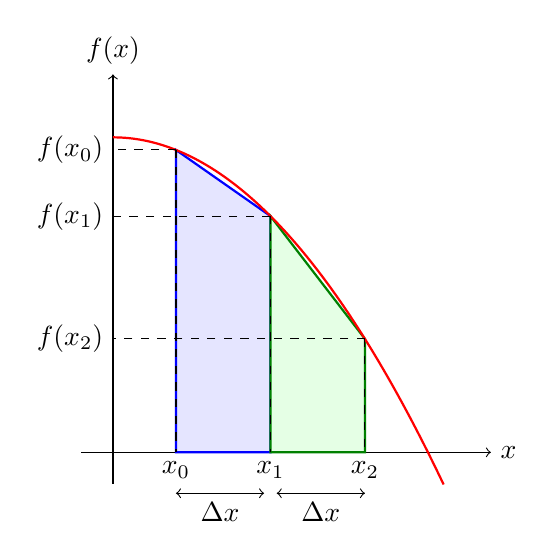
\begin{tikzpicture}[scale=4]
        % Axes
        \draw[->] (-0.1,0) -- (1.2,0) node[right] {$x$};
        \draw[->] (0,-0.1) -- (0,1.2) node[above] {$f(x)$};

        % Points
        \def\xa{0.2}
        \def\xb{0.5}
        \def\xc{0.8}
        
        % Valeurs de la fonction f(x) = -x^2 + 1
        \def\fa{0.96}
        \def\fb{0.75}
        \def\fc{0.36}

        % Trapèzes
        \fill[blue!10] (\xa,0) -- (\xa,\fa) -- (\xb,\fb) -- (\xb,0) -- cycle;
        \draw[blue, thick] (\xa,0) -- (\xa,\fa) -- (\xb,\fb) -- (\xb,0) -- cycle;

        \fill[green!10] (\xb,0) -- (\xb,\fb) -- (\xc,\fc) -- (\xc,0) -- cycle;
        \draw[green!50!black, thick] (\xb,0) -- (\xb,\fb) -- (\xc,\fc) -- (\xc,0) -- cycle;

        % Courbe
        \draw[thick, red, domain=0:1.05, samples=100] plot (\x, {-\x*\x + 1});

        % Projections
        \draw[dashed] (\xa, \fa) -- (\xa, 0) node[below] {$x_0$};
        \draw[dashed] (\xb, \fb) -- (\xb, 0) node[below] {$x_1$};
        \draw[dashed] (\xc, \fc) -- (\xc, 0) node[below] {$x_2$};
        
        \draw[dashed] (\xa, \fa) -- (0, \fa) node[left] {$f(x_0)$};
        \draw[dashed] (\xb, \fb) -- (0, \fb) node[left] {$f(x_1)$};
        \draw[dashed] (\xc, \fc) -- (0, \fc) node[left] {$f(x_2)$};

        % Distances
        \draw[<->] (\xa, -0.13) -- node[below] {$\Delta x$} (\xb-0.02, -0.13);
        \draw[<->] (\xb+0.02, -0.13) -- node[below] {$\Delta x$} (\xc, -0.13);
    \end{tikzpicture}
    \caption{Illustration of the trapezoidal rule for numerical integration. The integral is approximated as a sum of trapezoidal areas.}
    \label{fig:trapezoidal}
\end{figure}

%============================================================================
\section{Radon Transform and Connection to Abel Transform}
%============================================================================

\subsection{Physical Interpretation}

When a beam propagates through a medium, the measured intensity depends on the integral of the medium's properties along the beam's path. This fundamental principle is modeled by the Radon transform.

\subsection{Definition of the Radon Transform}

Consider an arbitrary 2D function $f(x,y)$ and a beam traversing it along a straight line. To define this line, we use two parameters:
\begin{itemize}
    \item $\theta$: the angle of observation
    \item $\rho$: the impact parameter (perpendicular distance from the origin to the line)
\end{itemize}

The geometric equation of the line is:
\begin{equation}
\rho = x\cos\theta + y\sin\theta
\end{equation}

We parameterize the coordinates $(x,y)$ along the ray using the coordinate $s$:
\begin{align}
x &= \rho \cos\theta - s \sin\theta \\
y &= \rho \sin\theta + s \cos\theta
\end{align}

The Radon transform measures the integral of $f(x,y)$ along the line:
\begin{equation}
\mathcal{R}[f(x,y)](\rho, \theta) = \int_{-\infty}^{+\infty} f(\rho \cos\theta - s \sin\theta, \rho \sin\theta + s \cos\theta) \, ds
\end{equation}

\subsection{Rotationally Symmetric Case}

For rotationally symmetric systems, the function depends only on the distance from the center:
\begin{equation}
r = \sqrt{x^2 + y^2} \quad \Rightarrow \quad f(x,y) = f(r)
\end{equation}

Since the object has circular cross-section, the projection is identical for all angles $\theta$. Choosing $\theta = 0$ simplifies the calculation:
\begin{equation}
\begin{cases}
x = \rho \\
y = s
\end{cases}
\end{equation}

The Radon integral becomes:
\begin{equation}
\mathcal{R}[f](\rho) = \int_{-\infty}^{+\infty} f\left(\sqrt{\rho^2 + s^2}\right) \, ds
\end{equation}

\subsection{Connection to Abel Transform}

Using symmetry:
\begin{equation}
\mathcal{R}[f](\rho) = 2 \int_0^{+\infty} f\left(\sqrt{\rho^2 + s^2}\right) \, ds
\end{equation}

Substituting $r^2 = \rho^2 + s^2$ and $ds = \frac{r \, dr}{\sqrt{r^2 - \rho^2}}$:
\begin{equation}
\mathcal{R}[f](\rho) = 2 \int_{\rho}^{+\infty} \frac{f(r) \, r}{\sqrt{r^2 - \rho^2}} \, dr
\end{equation}

This expression is precisely the Abel transform! The Radon transform of a rotationally symmetric function is equivalent to the Abel transform of the radial profile.
\section{Slow Varying Approximation, Extended Nonlinear Schrödinger Equation}

We start by writing the Maxwell equations in a gaseous dielectric medium, specifically air (a mixture of $N_2$ and $O_2$), taking into account the free charge sources (plasma and ions) generated by the intense laser pulse.
\begin{align}
\operatorname{Rot} \vec{B} &= \mu_0 \left( \vec{j} + \frac{\partial \vec{D}}{\partial t} \right) \\
\operatorname{Rot} \vec{E} &= -\frac{\partial \vec{B}}{\partial t} \\
\operatorname{div} \vec{B} &= 0 \\
\operatorname{div} \vec{D} &= 0
\end{align}

We can express the displacement vector by separating its linear and non-linear components. The linear part accounts for the material's dispersion via the frequency-dependent relative permittivity $\varepsilon(\omega)$:
\begin{align}
\vec{D}(\omega, r) &= \varepsilon_0 \vec{E}(\omega, r) + \vec{P}(\omega, r) \nonumber \\
&= \varepsilon_0 \vec{E} + \vec{P}_L + \vec{P}_{NL} \nonumber \\
&= \varepsilon_0 \left(1 + \chi^{(1)}\right) \vec{E} + \vec{P}_{NL} \nonumber \\
&= \varepsilon_0 \varepsilon(\omega) \vec{E}(\omega) + \vec{P}_{NL}(\omega) \nonumber \\
&= \vec{D}_{lin} + \vec{P}_{NL}
\end{align}

Let's derive the propagation equation by applying the curl operator ($\operatorname{Rot}$) to Faraday's law of induction. Using the vector identity $\operatorname{Rot}(\operatorname{Rot} \vec{E}) = \operatorname{grad}(\operatorname{div} \vec{E}) - \nabla^2 \vec{E}$, and assuming no macroscopic free charges alter the divergence of the electric field ($\operatorname{div}\vec{E} = 0$), we obtain:
\begin{equation}
\operatorname{Rot}(\operatorname{Rot}(\vec{E})) = \underbrace{\cancel{\operatorname{grad}(\operatorname{div}(\vec{E}))}}_{\text{No sources}} - \nabla^2 \vec{E} = -\frac{\partial}{\partial t} \operatorname{Rot} \vec{B} = -\mu_0 \frac{\partial \vec{j}}{\partial t} - \mu_0 \frac{\partial^2 \vec{D}}{\partial t^2}
\end{equation}

This yields the fundamental wave equation:
\begin{equation}
\nabla^2 \vec{E} = \mu_0 \frac{\partial^2}{\partial t^2} \vec{D}_{lin} + \mu_0 \frac{\partial^2}{\partial t^2} \vec{P}_{NL} + \mu_0 \frac{\partial \vec{j}}{\partial t}
\end{equation}

We separate the Laplacian into two parts: one along the propagation axis $z$, and the other along the orthogonal transverse axes ($\nabla_\perp^2$). The current density $\vec{j}$ is split into plasma and ion contributions:
\begin{equation}
\left( \frac{\partial^2}{\partial z^2} + \nabla_\perp^2 \right) \vec{E} = \frac{1}{c^2} \frac{\partial^2}{\partial t^2} \vec{D}_{lin} + \mu_0 \frac{\partial^2}{\partial t^2} \vec{P}_{NL} + \mu_0 \frac{\partial}{\partial t} (\vec{j}_{plasma} + \vec{j}_{ions})
\end{equation}

\subsection*{The Slow Varying Envelope Approximation (SVEA)}
We express the electric field as a highly oscillating carrier wave modulated by a slowly varying envelope $E$:
\begin{equation*}
\vec{E} = Ee^{i(k_{\omega}z-\omega t)}
\end{equation*}

Applying the second spatial derivative $\frac{\partial^2}{\partial z^2}$ to the field:
\begin{equation}
\frac{\partial^2 \vec{E}}{\partial z^2} = \left( \frac{\partial^2 E}{\partial z^2} + 2 i k_\omega \frac{\partial E}{\partial z} - k_\omega^2 E \right) e^{i(k_\omega z - \omega t)}
\end{equation}

Because the envelope $E$ varies spatially much slower than the wavelength of the carrier, we can safely neglect the second derivative of the envelope $\frac{\partial^2 E}{\partial z^2}$ compared to the first derivative term $2 i k_\omega \frac{\partial E}{\partial z}$. This is the Slow Varying Envelope Approximation. It yields:
\begin{equation}
\left( \nabla_\perp^2 + 2 i k_{\omega} \frac{\partial}{\partial z} - k_{\omega}^2 \right) \vec{E} = \frac{1}{c^2} \frac{\partial^2 \vec{D}_{lin}}{\partial t^2} + \mu_0 \frac{\partial^2 \vec{P}_{NL}}{\partial t^2} + \mu_0 \frac{\partial}{\partial t} (\vec{j}_p + \vec{j}_i)
\end{equation}

\subsection*{Linear Dispersion in the Fourier Domain}
The problem here is that the value $\vec{D}_{lin}$ is defined in the Fourier space. Because an ultrashort laser pulse possesses a broad spectrum, evaluating dispersion in the time domain requires a complex convolution ($D_{lin}(t) = \int \varepsilon(t-t') E(t') dt'$). To simplify the calculation, we apply the time derivative in the Fourier space (multiplying twice by $-i\omega$) and then perform an Inverse Fourier Transform.
\begin{align}
\frac{1}{c^2} \frac{\partial^2}{\partial t^2} \int_{-\infty}^{t} \varepsilon(t-t') E(r, t', z) dt' &\xrightarrow{\quad \mathcal{F} \quad} \frac{1}{c^2} \times (-i\omega)^2 \varepsilon(\omega) E(\omega, r) \nonumber \\
&= -\frac{\omega^2 \varepsilon(\omega)}{c^2} E(\omega, r) \nonumber \\
&= -\frac{\omega^2 n^2(\omega)}{c^2} E(\omega, r) \nonumber \\
&= -k^2(\omega) E(\omega, r)
\end{align}

We Taylor-expand the wave vector $k(\omega)$ around the central frequency ($\Omega = \omega - \omega_{central}$):
\begin{equation*}
k(\omega) \simeq k_{\omega} + k'_w \Omega + \frac{k''_w}{2} \Omega^2
\end{equation*}

Squaring this and neglecting higher-order terms:
\begin{align}
-k^2(\omega) \vec{E}(\omega, r) &\simeq -\left( k_{\omega} + k'_w \Omega + \frac{k''_w}{2} \Omega^2 \right)^2 \vec{E}(\omega, r) \nonumber \\
&= -\left[ k_{\omega}^2 + 2 k_{\omega} k'_w \Omega + k_{\omega} k''_w \Omega^2 \right] \vec{E}(\omega, r)
\end{align}

Transforming back to the time domain by replacing $\Omega \rightarrow i \frac{\partial}{\partial t}$ and $\Omega^2 \rightarrow -\frac{\partial^2}{\partial t^2}$:
\begin{equation}
\xrightarrow{\mathcal{F}^{-1}} -\left(k_{\omega}^2 + 2 i k_{\omega} k'_w \frac{\partial }{\partial t} - k_{\omega} k''_w \frac{\partial^2 }{\partial t^2} \right) \vec{E}
\end{equation}

Substituting this back into the SVEA equation (the $-k_{\omega}^2 E$ terms cancel out) and isolating $\frac{\partial E}{\partial z}$:
\begin{align}
\nabla_\perp^2 \vec{E} + 2 i k_{\omega} \frac{\partial \vec{E}}{\partial z} + 2 i k_{\omega} k'_w \frac{\partial \vec{E}}{\partial t} - k_{\omega} k''_w \frac{\partial^2 \vec{E}}{\partial t^2} = \mu_0 \frac{\partial^2 \vec{P}_{NL}}{\partial t^2} + \mu_0 \frac{\partial}{\partial t} [\vec{j}_{plasma} + \vec{j}_{ions}] \nonumber \\
\frac{\partial \vec{E}}{\partial z} = \frac{i}{2 k_{\omega}} \nabla_\perp^2 \vec{E} - \left( k'_w \frac{\partial}{\partial t} + \frac{i k''_w}{2} \frac{\partial^2}{\partial t^2} \right)\vec{E} - \frac{i \mu_0}{2 k_{\omega}} \frac{\partial^2 \vec{P}_{NL}}{\partial t^2} - \frac{i \mu_0}{2 k_{\omega}} \frac{\partial}{\partial t} [\vec{j}_{plasma} + \vec{j}_{ions}]
\end{align}

\subsection*{Nonlinear Contribution: The Optical Kerr Effect}
In a centrosymmetric medium like air, the second-order susceptibility $\chi^{(2)}$ is exactly zero. The primary nonlinearity is therefore the third-order effect.
\begin{equation*}
\vec{P} = \varepsilon_0 \chi^{(1)}\vec{E}  + \underbrace{\cancel{\varepsilon_0 \chi^{(2)} \vec{E}^2}}_{\text{Centrosymmetric}} + \varepsilon_0 \chi^{(3)} \vec{E}^3 + \dots
\end{equation*}

We isolate the component oscillating at the fundamental frequency $\omega$ (Optical Kerr Effect) and neglect the $3\omega$ term (Third Harmonic Generation), as it is heavily phase-mismatched and cannot accumulate energy during propagation.
\begin{equation}
\vec{P}_{NL}=\varepsilon_0 \chi^{(3)} \vec{E}^3 = \underbrace{\frac{3}{4} \varepsilon_0 \chi^{(3)}_{(\omega)} |\vec{E}|^2 \vec{E} \cos(\omega t)}_{\substack{\text{Kerr Effect} \\ \vec{P}_{NL} \swarrow}} + \underbrace{\frac{|\vec{E}|^2 \vec{E}}{4} \varepsilon_0 \chi^{(3)}_{(3\omega)} \cos(3\omega t)}_{\text{THG (Neglected)}}
\end{equation}

Evaluating the source term for the equation:
\begin{equation}
- \frac{i \mu_0}{2 k_{\omega}} \frac{\partial^2 \vec{P}_{NL}}{\partial t^2} \approx i \frac{3}{8} \frac{\omega^2}{k_{\omega} c^2} \chi^{(3)}_{(\omega)} |\vec{E}|^2 \vec{E}
\end{equation}

\subsection*{Ionization Losses (PPT Model)}
High-intensity pulses lose energy by ionizing the gas. The real power $\mathcal{P}$ absorbed by the medium equates to the ionization potential $U_p$ multiplied by the ionization rate $W_{PPT}(E)$ and the molecular density $N_{mol}$. Knowing that $k_{\omega} = \frac{\omega}{c} n_{\omega}$:
\begin{align}
\mathcal{P} = \frac{1}{2} \operatorname{Re}(\vec{J}_{ion} \vec{E}^*) &= U_p N_{mol} W_{PPT}(E) \nonumber \\
J_{ion} &= \frac{2 U_p N_{mol} W_{PPT}(E) \vec{E}}{|\vec{E}|^2}
\end{align}

Evaluating the source term for the propagation equation with $\frac{\partial}{\partial t}\vec{J}_{ion} = -i\omega\vec{J}_{ion}$
\begin{equation}
- \frac{i \mu_0}{2 k_{\omega}} \frac{\partial \vec{J}_{ion}}{\partial t} = - \frac{U_p N_{mol} W_{PPT}(E)}{n_{\omega} \varepsilon_0 c |E|^2} E
\end{equation}

\subsection*{Plasma Contribution (Drude Model)}
Freed electrons form a plasma that interacts with the laser, causing energy absorption and beam defocusing. Using the Drude model, we determine the electron velocity $v$ influenced by the electric field and a collision time $\tau_c$:
\begin{equation*}
\left. \begin{aligned}
m_e \frac{\partial v}{\partial t} &= -e E - \frac{m_e}{\tau_c} v \\
- i \omega m_e v &= -e E - \frac{m_e v}{\tau_c}
\end{aligned} \right\} \implies v = \frac{-e E \tau_c}{m_e (1 - i \omega \tau_c)}
\end{equation*}

The macroscopic plasma current is $\vec{J}_{plasma} = -e N_p^e v$:
\begin{equation}
\vec{J}_{plasma} = \frac{e^2 N_p^e \tau_c (1 + i \omega \tau_c)}{m_e (1 + \omega^2 \tau_c^2)}\vec{E}
\end{equation}

Evaluating the source term and identifying the inverse Bremsstrahlung cross-section $\sigma_{\omega}$:
\begin{align}
- \frac{i \mu_0}{2 k_{\omega}} \frac{\partial \vec{J}_{plasma}}{\partial t} &= - \frac{\mu_0 e^2 N_p^e \tau_c (1 + i \omega \tau_c) \omega \vec{E}}{m_e (1 + \omega^2 \tau_c^2)} \nonumber \\
&= - \frac{1}{2} \frac{e^2 \tau_c}{\varepsilon_0 n_{\omega} c m_e (1 + \omega^2 \tau_c^2)} (1 + i \omega \tau_c) N_p^e \vec{E}
\end{align}
With $\omega^2\tau_c^2 \gg 1$ and $n_{\omega}\omega = k_{\omega}c$
\begin{align}
- \frac{i \mu_0}{2 k_{\omega}} \frac{\partial \vec{J}_{plasma}}{\partial t} &= - \frac{1}{2} \underbrace{\frac{e^2}{\varepsilon_0 k_{\omega} m_e c^2 \omega \tau_c}}_{\text{Bremsstrahlung CS } \equiv \sigma_w} (1 + i \omega \tau_c) N_p^e \vec{E}\\
&- \frac{i \mu_0}{2 k_{\omega}} \frac{\partial \vec{J}_{plasma}}{\partial t}= - \frac{\sigma_{\omega}}{2} (1 + i \omega \tau_c) N_p^e \vec{E}
\end{align}


\subsection*{Final Equation for the Air Mixture}
Since air is a mixture, the Kerr, plasma, and ion terms must be summed over its primary constituents ($O_2$ and $N_2$). Additionally, the neutral molecules available for the Kerr effect and ionization deplete as electrons are stripped. The remaining neutral density is the initial density $N_p$ minus the free electron density $N_p^e$.

The final Extended Nonlinear Schrödinger Equation is:
\begin{align}
\frac{\partial \vec{E}}{\partial z} &= \frac{i}{2 k_{\omega}} \nabla_\perp^2 \vec{E} - \left( k'_w \frac{\partial}{\partial t} + i \frac{k''_w}{2} \frac{\partial^2}{\partial t^2} \right) \vec{E} \nonumber \\
&\quad + \sum_{p=O_2, N_2} \frac{N_p - N_p^e}{N_{mol}} \left[ i \frac{3}{8} \frac{\omega^2}{k_{\omega} c^2} \chi^{(3)}_{(\omega)} |\vec{E}|^2 - \frac{U_p N_{mol} W_{PPT}(E)}{n_{\omega} \varepsilon_0 c |\vec{E}|^2} \right] \vec{E} \nonumber \\
&\quad - \sum_{p=O_2, N_2} \frac{\sigma_{\omega}}{2} (1 + i \omega \tau_c) N_p^e \vec{E}
\end{align}

\subsection*{Electron Density Evolution}
To close the system, we need the evolution of the free electron density $N_p^e$. It grows through two mechanisms: direct photoionization of remaining neutrals (PPT), and avalanche ionization (where the plasma absorbs energy, accelerating electrons to knock out further electrons).

\begin{equation}
\frac{d N_p^e}{dt} = \underbrace{(N_p - N_p^e) W_{PPT}(E)}_{\text{Direct Photoionization}} \quad + \quad \underbrace{\frac{\sigma_{\omega} I N_p^e}{U_p}}_{\text{Avalanche Ionization}}
\end{equation}

Expressing the laser intensity $I = \frac{1}{2} n_{\omega} \varepsilon_0 c |E|^2$, we get the final rate equation:
\begin{equation}
\frac{d N_p^e}{dt} = (N_p - N_p^e) W_{PPT}(E) + \frac{\sigma_{\omega} N_p^e}{2 U_p} n_{\omega} \varepsilon_0 c |E|^2
\end{equation}
%============================================================================
\section{References}
%============================================================================

\begin{thebibliography}{99}

\bibitem{gonzalez2012plasma} 
Dr. Bruno Gonzalez-Izquierdo, Dr. Haruyuki Sakurai, Dr. Kuniaki Konishi and Prof. Junji Yumoto. 
``Plasma electron density and plasma temperature characterization in air and solid targets: Interferometry and Shadowgraphy.'' 
\textit{Journal of Applied Physics}, 2012.

\bibitem{tatum2020stellar}
Jeremy Tatum. 
``University of Victoria, Stellar Atmospheres, Chapter 8.6, page 139: Saha's Equation.''
2020.

\bibitem{cuni2020interference}
Collection of Solved Problems in Physics. 
``Task 1966: Interference of Two Plane Waves Propagating in Different Directions.'' 
Department of Physics Education, Faculty of Mathematics and Physics, Charles University in Prague.
\newline
\url{https://physicstasks.eu/}

\bibitem{takeda1982fourier}
Mitsuo Takeda, Hideki Ina and Seiji Kobayashi. 
``Fourier-transform method of fringe-pattern analysis for computer-based topography and interferometry.'' 
\textit{Journal of the Optical Society of America}, vol. 72, no. 1, pp. 156--160, 1982.
\newline
University of Electrocommunications, 1-5-1 Chofugaoka, Chofu, Tokyo 182, Japan.

\bibitem{Leith}
Emmett N. Leith and Juris Upatnieks, ''Reconstructed Wavefronts and Communication Theory*.'' 
\textit{Journal of the Optical Society of America} vol. 52, 1123-1130 (1962)
\url{https://opg.optica.org/josa/fulltext.cfm?uri=josa-52-10-1123}
\end{thebibliography}

\end{document}
